\section{Diagramme d'états-transitions}

	\subsection{Planification}
		\begin{figure}
			\begin{center}
				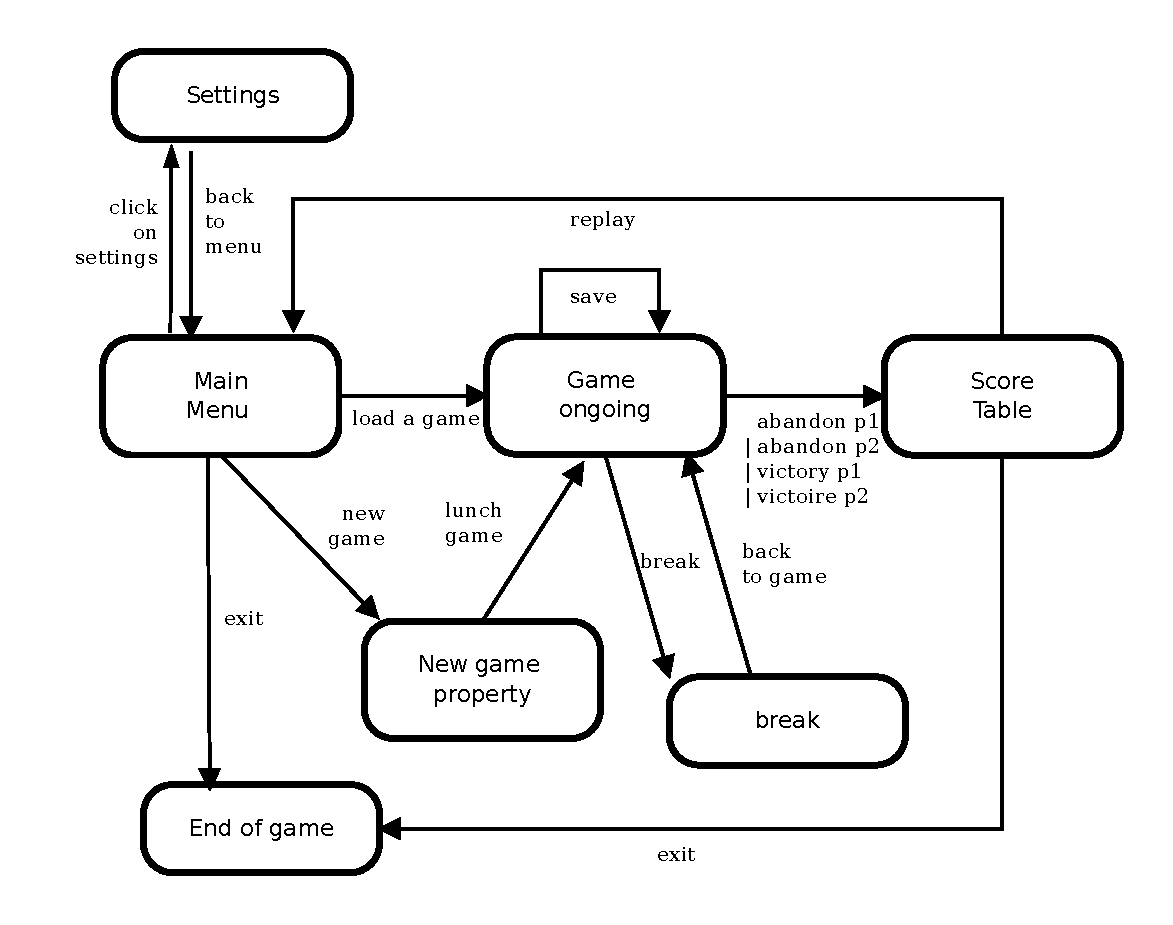
\includegraphics[width=1\textwidth]{figure/etat_transition_partie.pdf}
			\end{center}
			\caption{Diagrame d'états-transitions}
			\label{fig:planif}
		\end{figure}

		Nunc ut fermentum orci. Donec congue fringilla arcu id dapibus. Mauris aliquam vestibulum nisi, et euismod lacus convallis ut. Nullam nec justo a odio pretium aliquet. Vestibulum commodo porta enim. Vivamus consectetur, metus et aliquet accumsan, sem augue efficitur sem, id placerat metus odio a mauris. Donec id auctor mauris. Vestibulum ante ipsum primis in faucibus orci luctus et ultrices posuere cubilia Curae; Morbi felis diam, accumsan condimentum fringilla id, ultrices a neque. Vivamus sit amet odio quis nisi cursus congue sed vel magna. Pellentesque ac elit dapibus, feugiat massa vitae, ultrices massa. Cras quis turpis interdum, facilisis elit viverra, sollicitudin sem.

		Quisque aliquam enim vel dui tempor accumsan. Nulla facilisi. Morbi sit amet libero nisi. Nullam vel augue non erat lobortis viverra. Nunc dapibus volutpat lorem eu elementum. Donec ut egestas lorem. Donec fermentum dapibus volutpat. Pellentesque justo libero, dapibus at purus non, facilisis luctus dolor. 
